\documentclass[12pt,a4paper]{article}
%-------------------------------------------
%---Packages--------------------------------
%-------------------------------------------
\usepackage[utf8]{inputenc}
%\usepackage[T1]{fontenc}
%\usepackage{txfonts}
\usepackage{amsmath}
\usepackage{amsthm}
\usepackage{amsfonts}
\usepackage{array}
\usepackage{amssymb}
\usepackage{blindtext}
\usepackage{caption}
\usepackage{color}
\usepackage{csquotes}	    %
\usepackage{enumitem}	    %pour mieux bosser avec les listes. ajoute option label
\usepackage[yyyymmdd]{datetime}        %pour définir date custom
\usepackage{etaremune}
\usepackage{environ}
\usepackage{fancybox}
\usepackage{fancyhdr} 	    % Custom headers and footers
\usepackage{fancyref}
%\usepackage{float}
\usepackage{floatrow}       %float and floatrow can't be together...
\usepackage{gensymb}
\usepackage{graphicx}
\usepackage[colorlinks=true, linkcolor=purple, citecolor=cyan]{hyperref}
\usepackage{footnotebackref}
\usepackage{lipsum}
\usepackage{mathtools}
\usepackage{multicol}	    %gérer plusieurs colonnes
\usepackage{setspace}
\usepackage{subcaption}
\usepackage{todonotes}	    %Bonne gestion des TODOs
%TODO commenté pour tester l'utilité... à voir% \usepackage[tc]{titlepic}      %Permet de mettre une image en page de garde
\usepackage{tikz}	    % Pour outil de dessin puissant
\usepackage{ulem}	    %underline sur plusieurs lignes (avec \uline{})
\usepackage{vmargin} 	    %gestion des marges, avec dans l'ordre : gauche, haut, droit, bas, en-tête, entre en-tête et texte, bas de page, hauteur entre bas de page et texte
\usepackage{wrapfig}
\usepackage{xcolor}
\usepackage{xparse}                    %Pour utiliser NewDocumentCommand et des arguments 'mmooo'
%\usepackage{fullpage} 	    %supprime toutes les marges allouées aux notes, aussi en haut et en bas

%\ExplSyntaxOn
\pagestyle{fancyplain}	    %Makes all pages in the document conform to the custom headers and footers

%-------------------------------------------
%---Document Commands-----------------------
%---------------------------{----------------
\NewDocumentCommand{\framecolorbox}{oommm}
 {% #1 = width (optional)
  % #2 = inner alignment (optional)
  % #3 = frame color
  % #4 = background color
  % #5 = text
  \IfValueTF{#1}%
   {\IfValueTF{#2}%
    {\fcolorbox{#3}{#4}{\makebox[#1][#2]{#5}}}%
    {\fcolorbox{#3}{#4}{\makebox[#1]{#5}}}%
   }%
   {\fcolorbox{#3}{#4}{#5}}%
 }%
%------------------------------------------------
%------------------ENGLISH----------------------
%----------------------------------------------

\NewDocumentCommand{\epflTitle}{mO{Olivier Cloux}O{\today}O{Notes de Cours en}D<>{../../Common}}%Arguments : Matière, Auteur, Date, Titre du doc
{
\begin{titlepage}
    \vspace*{\fill}
    \begin{center}
        \normalfont \normalsize
        \textsc{Ecole Polytechnique Fédérale de Lausanne} \\ [25pt] % Your university, school and/or department name(s)
        \textsc{#4} %Titre du doc
        \\ [0.4 pt]
        \horrule{0.5pt} \\[0.4cm] % Thin top horizontal rule
        \huge #1 \\ % Matière
        \horrule{2pt} \\[0.5cm] % Thick bottom horizontal rule
        
\includegraphics[width=8cm]{#5/EPFL_logo}
        ~\\[0.5 cm]
        \small\textsc{#2}\\[0.4cm]
        \small\textsc{#3}\\
        ~\\
        ~\\
        
\includegraphics[scale=0.5]{#5/creativeCommons}
    \end{center}
    \vspace*{\fill}
\end{titlepage}
}


%-------------------------------------------
%-------------MATH NEW COMMANDS-------------
%-------------------------------------------
\newcommand{\somme}[2]{\ensuremath{\sum\limits_{#2}^{#1}}}
\newcommand{\produit}[2]{\ensuremath{\prod\limits_{#2}^{#1}}}
\newcommand{\limite}{\lim\limits_}
\newcommand{\llimite}[3]{\limite{\substack{#1 \\ #2}}\left(#3\right)}	%limites à deux condiitons
\newcommand{\et}{\mbox{ et }}
\newcommand{\deriv}[1]{\ensuremath{\, \mathrm d #1}}	%sigle dx, dt,dy... des dérivées/intégrales
%\newcommand{\fx}{\ensuremath{f'(\textbf{x}_0 + h}}
\newcommand{\ninf}{\ensuremath{n \to \infty}}	       %pour les limites : n tend vers l'infini
\newcommand{\xinf}{\ensuremath{x \to \infty}}	       %pour les limites : x tend vers l'infini
\newcommand{\infint}{\ensuremath{\int_{-\infty}^{\infty}}}
\newcommand{\xo}{\ensuremath{x \to 0}}									%x to 0
\newcommand{\no}{\ensuremath{n \to 0}}									%n zéro
\newcommand{\xx}{\ensuremath{x \to x}}									%x to x
\newcommand{\Xo}{\ensuremath{x_0}}										%x zéro
\newcommand{\X}{\ensuremath{\mathbf{X}} }
\newcommand{\A}{\ensuremath{\mathbf{A}} }
\newcommand{\R}{\ensuremath{\mathbb{R}} }								%ensemble de R
\newcommand{\rn}{\ensuremath{\mathbb{R}^n} } 							%ensemble de R de taille n
\newcommand{\Rm}{\ensuremath{\mathbb{R}^m} }  							%ensemble de R de taille m
\newcommand{\C}{\ensuremath{\mathbb{C}} }
\newcommand{\N}{\ensuremath{\mathbb{N}} }
\newcommand{\Z}{\ensuremath{\mathbb{Z}} }
\newcommand{\Q}{\ensuremath{\mathbb{Q}} }
\newcommand{\rtor}{\ensuremath{\R \to \R} }
\newcommand{\pour}{\mbox{ pour }}
\newcommand{\coss}[1]{\ensuremath{\cos\(#1\)}}						%cosinus avec des parenthèses de bonne taille (genre frac)
\newcommand{\sinn}[1]{\ensuremath{\sin\(#1\)}}					%sinus avec des parentèses de bonne taille (genre frac)
\newcommand{\txtfrac}[2]{\ensuremath{\frac{\text{#1}}{\text{#2}}}}		%Fractions composées de texte
\newcommand{\evalfrac}[3]{\ensuremath{\left.\frac{#1}{#2}\right|_{#3}}}
\renewcommand{\(}{\left(}												%Parenthèse gauche de taille adaptive
\renewcommand{\)}{\right)}
\newcommand{\longeq}{=\joinrel=}												%Parenthèse droite de taille adaptive


%-------------------------------------------------------
%------------------MISC NEW COMMANDS--------------------
%-------------------------------------------------------
\newcommand{\degre}{\ensuremath{^\circ}}
%\newdateformat{\eudate}{\THEYEAR-\twodigit{\THEMONTH}-\twodigit{\THEDAY}}



%-------------------------------------------------------
%------------------TEXT NEW COMMANDS--------------------
%-------------------------------------------------------
\newcommand{\ts}{\textsuperscript}
\newcommand{\evid}[1]{\textbf{\uline{#1}}}        %mise en évidence (gras + souligné)



%\newcommand{\Exemple}{\underline{Exemple}}
\newcommand{\Theoreme}{\underline{Théorème}}
\newcommand{\Remarque}{\underline{Remarque}}
\newcommand{\Definition}{\underline{Définition} }
\newcommand{\skinf}{\sum^{\infty}_{k=0}}
\newcommand{\combi}[2]{\ensuremath{\begin{pmatrix} #1 \\ #2 \end{pmatrix}}}	%combinaison parmi 1 de 2
\newcommand{\intx}[3]{\ensuremath{\int_{#1}^{#2} #3 \deriv{x}}}				%intégrale dx
\newcommand{\intt}[3]{\ensuremath{\int_{#1}^{#2} #3 \deriv{t}}}				%intégrale dy
\newcommand{\misenforme}{\begin{center} Mis en forme jusqu'ici\\ \line(1,0){400}\\ normalement juste, mais à améliorer depuis ici\end{center}}	%raccourci pour mise en forme
\newcommand*\circled[1]{\tikz[baseline=(char.base)]{
            \node[shape=circle,draw,inner sep=1pt] (char) {#1};}}			%pour entourer un chiffre
\newcommand{\horrule}[1]{\rule{\linewidth}{#1}} 				% Create horizontal rule command with 1 argument of height

\theoremstyle{definition}
\newtheorem{exemp}{Exemple}
\newtheorem{examp}{Example}


%-------------------------------------------
%---Environments----------------------------
%-------------------------------------------
\NewEnviron{boite}[1][0.9]{%
	\begin{center}
		\framecolorbox{red}{white}{%
			\begin{minipage}{#1\textwidth}
 	 			\BODY
			\end{minipage}
		}
	\end{center}
}
\NewEnviron{blackbox}[1][0.9]{%
	\begin{center}
		\framecolorbox{black}{white}{%
			\begin{minipage}{#1\textwidth}
 	 			\BODY
			\end{minipage}
		}
	\end{center}
}
\NewEnviron{exemple}[1][0.8]{%
    \begin{center}
        \framecolorbox{white}{gray!20}{%
            \begin{minipage}{#1\textwidth}
                \begin{exemp}
                    \BODY
                \end{exemp}
            \end{minipage}
        }
    \end{center}
}
\NewEnviron{suiteExemple}[1][0.8]{%
    \begin{center}
        \framecolorbox{white}{gray!20}{%
            \begin{minipage}{#1\textwidth}
                \BODY
            \end{minipage}
        }
    \end{center}
}
\NewEnviron{colExemple}[1][0.8]{%
    \begin{center}
        \framecolorbox{white}{gray!20}{%
            \begin{minipage}{#1\columnwidth}
                \begin{exemp}
                    \BODY
                \end{exemp}
            \end{minipage}
        }
    \end{center}
}
\NewEnviron{example}[1][0.8]{%
    \begin{center}
        \framecolorbox{white}{gray!20}{%
            \begin{minipage}{#1\textwidth}
                \begin{examp}
                    \BODY
                \end{examp}
            \end{minipage}
	}
    \end{center}
}
\NewEnviron{systeq}[1][l]{
			\begin{center}
				$\left\{\begin{array}{#1}
					\BODY
				\end{array}\right.$
			\end{center}
 }





%-------------------------------------------
%---General settings-----------------------
%-------------------------------------------
\renewcommand{\headrulewidth}{1pt}										%ligne au haut de chaque page
\renewcommand{\footrulewidth}{1pt}										%ligne au pied de chaque page
\setstretch{1.6}
\author{Olivier Cloux}

\usepackage[tc]{titlepic}
\usepackage{graphicx}

\newcommand{\zn}{\ensuremath{(z_n)} }
\newcommand{\nz}{\overline{z}}
\renewcommand{\contentsname}{Table des Matières}
%%%%%%%%%%%%%%%%%%%%%%%%%%%%%%%%%%%%%%%%%%
%TODO : Supprimer quand plus de todo %%%%%
\marginparwidth = 75pt
\textwidth = 400pt
%%%%%%%%%%%%%%%%%%%%%%%%%%%%%%%%%%%%%%%%%%%%
\begin{document}
\setstretch{1}
\epflTitle{Analyse IV}[Olivier Cloux][Automne 2015]
\newpage
\tableofcontents
\setstretch{1.2}
\newcommand{\dive}{\text{ div }}
\newcommand{\rot}{\text{ rot }}
\newcommand{\grad}{\text{ grad }}
\section{Nombres complexes}
\subsection{Définitions et propriétés}
\begin{boite}[0.7]
	\centering
	On définit $\C = \{x,y \in \R : x + y\cdot i = z\}$ avec $i^2 = -1$
\end{boite}
Soient $x_1,x_2,y_2,y_2 \in \R$. Nous posons l'addition et la multiplication dans $\C$ ainsi :
\begin{itemize}
	\item 	Addition :
			\begin{equation}
				(x_1 + i\cdot y_2) + (x_2 + i \cdot y_2) = (x_1+x_2) + i\cdot(y_1+y_2)
			\end{equation}
	\item 	Multiplication : 
			\begin{equation}
				(x_1 + i\cdot y_2) \cdot (x_2 + i \cdot y_2) = (x_1x_2-y_1y_2) + i\cdot(x_1y_2 + x_2y_1)
			\end{equation}
\end{itemize}
Une fois ces points définis, les propriétés suivantes s'appliquent $\forall z_1,z_2,z_3 \in \C$ :
\begin{itemize}
	\item 	Associativité pour l'addition :
			\begin{equation}
				z_1 + (z_2 + z_3) = (z_1+z_2) + z_3
			\end{equation}
	\item 	Commutativité :
			\begin{equation}
				z_+ z_2 = z_2 + z_1
			\end{equation}
	\item	Associativité pour la multiplication :
			\begin{equation}
				z_1(z_2z_3) = (z_1z_2)z_3
			\end{equation}
	\item 	Distributivité :
			\begin{equation}
				(z_1 + z_2)z_3 = z_1z_3 + z_2z_3
			\end{equation}
\end{itemize}
Finalement, nous définissons la \textbf{partie réelle} d'un nombre $z$ comme $x$, soit la partie sans $i$ ; la partie réelle s'écrit $Re\{z\}$. Inversement, la partie imaginaire correspond à toute partie comprenant des $i$ ; celle-ci s'écrit $Im\{z\}$
\begin{exemple}[0.85]
	Soit 
	\[z = (1+2i)^2 = 1^2 + 2\cdot 1 \cdot 2i + (2i)^2 = 1 + (2^2 \cdot i^2) + 4i = 1 - 4 + 4i = -3 + 4\cdot i\]
	Ainsi, $Re\{z\} = -3$ et $Im\{z\} = 4$
\end{exemple}
\subsubsection{Conjugué}
Une fois les nombres complexes définis, nous cherchons à définir un ``opposé'' de manière a annuler la partie imaginaire d'un nombre en l'additionnant avec son conjugué. Nous posons alors $\overline{z}$ le \textbf{conjugué} de $z$ ainsi :
\begin{equation}
	z = x + i\cdot y \iff \overline{z} = x - i\cdot y
\end{equation}
Nous avons ainsi les deux propriétés suivantes :
\begin{align}
	\overline{z_1 + z_2} = \overline{z_1} + \overline{z_2}\\
	\overline{z_1\cdot z_2} = \overline{z_1}\cdot\overline{z_2}
\end{align}

\subsubsection{Module}
On définit le \textbf{module} de $z$ comme 
\begin{equation}
	|z| = \sqrt{x^2 + y^2} = \sqrt{z \cdot \overline{z}}
\end{equation}
\uline{Démonstration : Appendice \ref{app_preuve: module}}.

Par inégalité triangulaire (puis par récurrence) on a que 
\begin{align}
	|z_1 + z_2| \leq |z_1| + |z_2|\\
	|z_1 + ... + z_k| \leq |z_1| + ... + |z_k|
\end{align}
\uline{Démonstration} : Appendice \ref{app_preuve: inegalite triangulaire}

Finalement, 3 propriétés utiles :
\begin{equation}
	-|z| \leq Re\{z\} \qquad |z| \leq Im\{z\} \qquad |z_1z_2| = |z_1|\cdot|z_2|
\end{equation}

\subsubsection{Inverse}
Avec les nombres réels, nous avons défini l'inverse, tel que le multiple d'un nombre et de son inverse donne toujours 1. Nous pouvons faire le même démarche avec les nombres complexes. En supposant que $z \in \C\setminus\{0\}$, on a 
\begin{equation}
	\frac{1}{z} = \frac{\overline{z}}{|z|} = \frac{x-i\cdot y}{x^2 + y^2} \text{ tel que }z \cdot \frac{1}{z} = 1
\end{equation}
Cela nous donne deux propriétés :
\begin{equation}
	z_1 \cdot z_2 = 0 \to z_1 = 0\ \vee z_2 = 0 \qquad \et \qquad \overline{\(\frac{1}{z}\)} = \frac{1}{\overline{z}}
\end{equation}
\begin{exemple}
	\[\frac{1}{z} = \frac{1}{x+ i\cdot y} = \frac{x-i\cdot y}{x^2 + y^2}\]
	Alors : $Re\{z\} = \frac{x}{x^2 + y^2}$ et $Im\{z\} = \frac{-y}{x^2 + y^2}$
\end{exemple}

\subsection{Représentation géométrique}
\begin{figure}
	\centering
	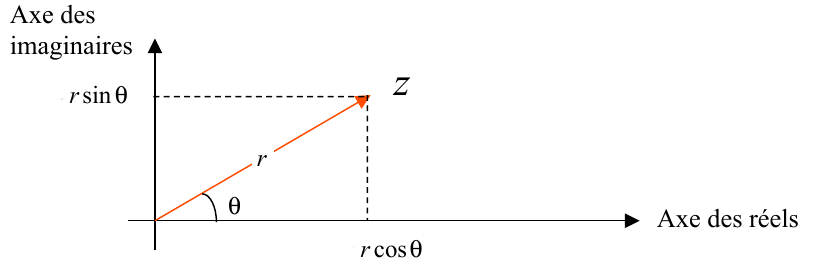
\includegraphics[scale=0.5]{images/geo_complexe}
	\caption{Représentation géométrique d'un complexe}
	\label{fig: repres geom complexe}
\end{figure}
Pour représenter les nombres réels, nous utilisons la droite des réels, sur laquelle nous plaçons tous les nombres à la suite. Mais cette représentation devient inutile avec les complexes : comment représenter deux nombres avec la même partie réelle mais deux parties imaginaires différentes ? Simplement, nous ajoutons une dimension à notre représentation. Nous parlons maintenant du \textbf{plan complexe}.

Ce plan est composé de deux axes : \uline{l'axe des réels} (pour représenter la partie réelle du nombre) et \uline{l'axe des imaginaires} (pour la partie imaginaire). Cette représentation ---visible à la figure \ref{fig: repres geom complexe}--- permet d'adapter nos notations et nos opérations.

\begin{boite}
On définit 
\[z = x + 1 \cdot y = r\cos(\theta) + i\cdot r\sin(\theta) = r(\cos(\theta) + i\cdot \sin(\theta)) = re^{i\theta}\]
Ainsi on pose $|z| = r$ et $arg(z) = \theta$, ce qui nous permet de lier précisément la géométrie et nos nombres.
\end{boite}
\subsubsection{Opérations}
Soient $z_1 = r_1(\cos\theta_1 + i\cdot \sin\theta_1)$ et $z_2 = r_2(\cos\theta_2 + i\cdot \sin\theta_2)$. Ainsi :
\begin{equation}
	z_1z_2 = r_1r_2\big(\cos(\theta_1 + \theta_2) + i\cdot \sin(\theta_1 + \theta_2)\big)
\end{equation}
On trouve alors facilement que 
\begin{equation}
	|z_1z_2| = |z_1|\cdot |z_2|  \et \arg(z_+\cdot z_2) = arg(z_1) + arg(z_2)
\end{equation}
Prenons maintenant : 
\begin{equation}
	\frac{z_1}{z_2} = \frac{r_1}{r_2}\big(\cos(\theta_1-\theta_2) + i\sin(\theta_1 - \theta_2)\big)
\end{equation}
De même : 
\begin{equation}
	\frac{1}{z_2} = \frac{1}{r_2}\big(\cos(-\theta_2) + i\sin(-\theta_2)\big)
\end{equation}

\subsubsection{Puissances et racines}
Soit $z = r(\cos\theta + i \sin\theta)$. Alors 
\begin{equation}
	z^n =r^n(\cos(n\theta) + i\sin(n\theta))
\end{equation}
Nous en déduisons la \textbf{formule de Moivre} :
\begin{equation}
	(\cos\theta + i\sin\theta)^n = \cos(n\theta) + i\sin(n\theta)
	\label{equ: moivre}
\end{equation}
La racine se définit inversement : Soit $z \in \C$, alors $w\in \C$ est défini comme la racine n-ème de $z$ si et seulement si $w^n = z$. Ainsi, pour $z \neq 0$, on cherche 
\[w = s(\cos\varphi + i\sin\varphi) \text{ tel que }s^n(\cos(n\varphi) + i\sin(n\varphi)) = r(\cos\theta + i\sin\theta)\]
Ce qui implique que 
\[s^n = r \to s = \sqrt{r} \et (\forall n \in \N)(\forall k \in \{0,...,n-1\}) : n\varphi = \theta + 2k\pi \to \varphi_k = \frac{\theta}{n} + \frac{2k\pi}{n}\]
Ainsi, on a 
\[\varphi_k = \varphi:k + n\pi \in \Z \et \varphi_n = \varphi_0 + 2\pi\]

\begin{exemple}
	Soit $z = \cos\frac{\pi}{2} + i\sin\frac{\pi}{2}$, on a alors deux racines : 
	\[\cos\frac{\pi}{4} + i\sin\frac{\pi}{4} \et \cos\frac{5\pi}{4} + i\sin\frac{5\pi}{4}\]
\end{exemple}
\begin{exemple}
Trouver toutes les racines 3\ts{èmes} de 1.\\
On a $1 = \cos\theta + i\sin\theta$, d'où \[w_0 = 1,\ w_1 = \coss{\frac{2\pi}{3}} + i\sinn{\frac{2\pi}{3}},\ w_2 = \coss{\frac{4\pi}{3}} + i\sinn{\frac{4\pi}{3}}\]
\end{exemple}

\subsection{Éléments sur la topologie}
\begin{boite}
	\evid{Définitions :}
	\begin{itemize}
		\item 	Une suite $(z_n) \subset \C$ converge vers $a \in \C$ ssi 
				\[(\forall \epsilon > 0)(\exists n_\epsilon) : n \geq n_\epsilon \vee |z_n - a| \leq \epsilon\]
		\item 	Une suite $(z_n) \subset \C$ est dite \textbf{de Cauchy} ssi 
		\[(\forall \epsilon > 0)(\exists n_\epsilon > 0)(\forall m,n > n_\epsilon) : |z_n - z_m| < \epsilon\]
	\end{itemize}
\end{boite}
\subsubsection*{Propriétés}
Soit $(z_n) \subset \C$, alors $(z_n$ converge ssi \zn est une suite de Cauchy \uline{Preuve Appendice \ref{app_preuve: converge cauchy}}

\subsubsection{Définitions}
\begin{itemize}
	\item 	Soit $a \in \C et r>0$, alors nous définissons la boule ouverte de rayon $r$ centrée en $a$ :
			\[B_r(a) = \{z\in \C : |z-a| < r\}\] 
	\item 	Soient $z_1,z_2 \in  \C$, alors 
			\[[z_1,z_2] = \{t \in [0,1] : \gamma(t) = (1-t)\cdot z_1 + t \cdot z_2\}\]
	\item 	Un ensemble $\Omega \subset \C$ est ouvert ssi \[(\forall a \in \Omega)(\exists r > 0) : B_r(a) \subset \Omega\]
	\item 	Un ensemble $D \subset \C$ est fermé ssi $\C \setminus D$ est ouvert
	\item 	Un ensemble $\Omega$ est dit une domaine de \C ssi $\Omega$ est ouvert et ($\forall z_1, z_2 \in \C) : \exists$ une courbe contenue dans $\Omega$ ; ainsi on pose $\gamma : [a,b] \to \Omega$ tq $\gamma(a) = z_1$ et $\gamma(b) = z_2$.
	\item 	$\Omega$ est dit convexe ssi $(\forall z_1,z_2 \in \Omega) : [z_1,z_2] \subset \Omega$
	\item 	Ainsi : Si $\Omega$ est convexe et ouvert, alors $\Omega$ est un domaine.
\end{itemize}
\begin{exemple}
	Si $|z| < 1$, montrer que $\frac{z}{1+z^n} \to z$\\
	On a que $|z^n| = |z|^n \to 0$ puisque $|z| < 1$, d'où $1+z^n \to 1$
\end{exemple}

\section{Fonctions holomorphes}
\setcounter{equation}{0}
\subsection{Limite et continuité d'une fonction complexe}
\begin{boite}
    \evid{Définition 2.1.1} Soit $\Omega \subset \C$ et une fonction $f : \Omega \to \C,\ z_0 \in \C$. On dit que $f$ a une limite $A$ en $z_0$ si $(\forall \epsilon > 0)(\exists \delta > 0) t.q. : |f(z) - A| < \epsilon$. Si $z \in \Omega$ et $0 \leq z-z_0| < \delta$
\end{boite}
\begin{exemple}~
    \begin{enumerate}[label=\alph*)]
        \item     $f(z) = z$ :$f$ a une limite $z_0\ \forall z_0 \in \C$
        \item     $f(z) = \overline{z}$ : $f$ a une limite : $\overline{z}_0\ \forall z_0 \in \C$ :
                  \[|f(z) - \overline{z}_0| = |\nz - \nz_0| = |z-z_0|\]
        \item     $f(z) = \left\{\begin{array}{ll}
                    z & z \neq 0\\
                    1 z = 0
                  \end{array}\right. :$ $f$ a une limite $z_0 : \forall z_0 \in \C$. Prenons $z_0 = 0$. La définition n'est pas atteignable. En revanche, pour $z \neq 0 : |f(z)| = |z|$.
    \end{enumerate}
\end{exemple}

\begin{boite}
    \evid{Définition 2.1.2} soit $\Omega \subset \C$ un ensemble ouvert, $z_0 \in \Omega$ et une fonction $f : \Omega \to \C$. On dit que \textbf{$f$ est continu en $z_0$} si et seulement si
    \begin{equation}
        \limite{z \to z_0}{f(z)} = f(z_0)
    \end{equation}
\end{boite}
\begin{exemple}
    Pour reprendre les exemples précédents :
    \begin{enumerate}[label=\alph*)]
        \item     $f$ est continu en $z_0\ \forall z_0 \in  \C$
        \item     idem
        \item    $f$ est continu en $z_0 \in C\setminus\{0\}$
    \end{enumerate}
\end{exemple}
\evid{Proposition 2.1.2 :} Supposons que $f$ et $g$ ont une limite en $z_0$ Alors :
\begin{enumerate}
    \item     $\limite{z \to z_0}(f+g)(z) =\limite{z \to z_0} f(z) + \limite{z \to z_0} g(z)$
    \item     $\limite{z \to z_0} (fg)(z) = \limite{z \to z_0}f(z) \cdot \limite{z \to z_0} g(z)$
    \item     $\limite{z \to z_0} \(\frac{f}{g}\)(z) = \frac{\limite{z \to z_0}f(z)}{\limite{z \to z_0} g(z)}$ si $\limite{z \to z_0}g(z) \neq 0$
\end{enumerate}

\evid{Remarque 1.2.1} \[\limite{z \to z_0} f(z) = A \iff \limite{z \to z_0} \overline{f(z)} = \overline{A} \iff \left\{\begin{array}{l}
    \limite{z \to z_0} Re(f(z)) = Re(A)\\
    \limite{z \to z_0} Im(f(z)) = Im(A)
\end{array}\right.\]

\subsection{Dérivée d'une fonction complexe}
\begin{boite}
    \evid{Définition 2.2.1 :} Soient $\Omega \subset \C$ un ensemble ouvert, $z_0 \in \C$ et une fonction $f : \Omega \to \C$. On dit que \textbf{$f$ est dérivable en $z_0$} si et seulement si la limite 
    \begin{equation}
        \limite{z \to z_0} \frac{f(z) - f(z_0)}{z-z_0} \quad \text{ existe}
    \end{equation}
\end{boite}
Dans ce cas $f'(z_0) = \limite{z \to z_0} \frac{f(z) - f(z_0)}{z-z_0}$ et on l'appelle \textit{la dérivée de $f$ en $z_0$}
\begin{exemple}
    Continuation des exemples précédents :
    \begin{enumerate}[label=\alph*)]
        \item     $\frac{f(z) - f(z_0)}{z-z_0} = \frac{z-z_0}{z-z_0} = 1$. Donc on note $f'(z_0) = 1$
        \item     $\frac{f(z) - f(z_0)}{z-z_0} = \frac{\nz - \nz_0}{z-z_0} = $ %TODO
    \end{enumerate}
\end{exemple}
\todo{il a écrit quoi ??}
\evid{Proposition 2.2.1 :} Supposons que $f$ et $g$ soient dérivables en $z_0$. Alors :
\begin{enumerate}
    \item     $f+g$ est dérivable en $z_0$ et : \[(f+g)'(z_0) = f'(z_0) + g'(z_0)\]
    \item     $fg$ est dérivable en $z_0$ et : \[(fg)'(z) = f'(z_0)g(z_0) + f(z_0)g'(z_0)\]
    \item     Si $g(z_0) \neq 0$ alors $\frac{f}{g}(z_0)$ est dérivable et : \[\(\frac{f}{g}\)'(z_0) = \frac{f'(z_0)g(z_0) - f(z_0)g'(z_0)}{g^2(z_0)}\]
    \item Si $f: \Omega \to U$ et $g: U \to \C$ et $f$ est dérivable en $z_0$ et $g$ est dérivable en $f(z_0)$. Alors :
    \[\big(g(f)\big)'(z_0) = g'\big(f(z_0)\big) f'(z_0)\]
\end{enumerate} 
\uline{Preuve :} c.f. Appendice \ref{app_preuve: operations derivee complexe}.

\evid{Corollaire 2.2.1 :} 
\begin{enumerate}
    \item     $(z^n)' = nz^{n-1}$
    \item     similaire avec d'autres domaines ? \todo{chercher dans notes} %TODO
\end{enumerate}
\evid{Proposition 2.2.2 :} Soit $f$ une fonction dérivable en $z$. Alors 
\begin{equation}
    f'(z) = \frac{\partial f}{\partial x}(x,y) =\frac{1 \cdot \partial}{i\cdot \partial y}f(x,y)
\end{equation}
\todo{compléter}
\evid{Corollaire 2.2.2 :} L'équation de Cauchy-Riemann : Soit $f$ une fonction dérivable en $z$. Nous posons $u = Re(f)$ et $v = Im(f)$. Alors : 
\todo{COMPLETER !}

\evid{Proposition 2.2.3 :} Si : $f$ est une fonction dérivable autour de $z$, $u,v$ sont de classe $C^2$ autour de $(x,y)$ . Alors $\Delta v = \Delta v = 0$ en $(x,y)$.
\begin{boite}
    \evid{Définition 2.2.3 :} Une fonction $u$ qui vérifie $\Delta u = 0$ est dite \textbf{harmonique}.
\end{boite}
\evid{Proposition 2.2.4} : Si $u$ et $v$ (réels) sont de classe $C^2$ et vérifient l'équation de Cauchy-Riemann (C-R), alors $f = u+v$ est dérivable.

\begin{boite}
    \evid{Définition :} $f: \Omega \to \C$. On dit que $f$ est holomorphe sur $\Omega$ si $f$ est dérivable en $z$, $\forall z \in \Omega$
\end{boite}

\evid{Proposition 2.2.5} si $u$ et $v$ sont de classe $C^2$ et $u$ et $v$ vérifient Cauchy-Riemann, nous définissons alors $f = u + iv$. $f$ est alors une fonction holomorphe. \\
\uline{Preuve :} Appendice \ref{app_preuve: proposition 2.2.5}

\begin{boite}
    \evid{Définition :} Soient $u$ est harmonique $(C^2)$. Alors $v$ est dite une fonction harmonique conjuguée de $u$ si $(CR)$ est valide.
\end{boite}
\evid{Exemple 2.2.5 :} vérifier que les fonctions suivantes sont harmoniques :
\begin{enumerate}
    \item     $u(x,y) = ax+by$
    \item     $u(x,y) = x^2-y^2$
    \item     $u(x,y) = e^x\sin(y)$
\end{enumerate}
\uline{Solution :}
\begin{enumerate}
    \item     $\Delta u = \frac{\partial^2 u }{\partial x^2} + \frac{\partial^2 u}{\partial y^2} = 0$
    \item     $\Delta u = 2-2 = 0$
    \item     $\Delta u = e^x\sin(y) - e^x\sin(y) = 0$
\end{enumerate}
\evid{Exemple 2.2.6 :} Soit $u(x,y) = x^2 + y^2$. Trouver une fonction harmonique conjuguée de $u$.\\
\uline{Solution :} 
\begin{align*}
    \left\{\begin{array}{l}
        \frac{\partial u}{\partial x} = 2x = \frac{\partial v}{\partial y}\\
        \frac{\partial u}{\partial y} = -2y = -\frac{\partial u}{\partial x}
    \end{array}\right.~ \\
    \to \frac{\partial v}{\partial y} = 2x \to v(x,y) = 2xy + g(x)\\
    \to \frac{\partial v}{\partial x} = 2y +  g'(y) = 2y \to g = \text{ const}
\end{align*}
Donc $v(x,y) = 2xy+c$ et nous voyons que:
\[u+iv = x^2 -y^2 + i2xy + ic = (x+iy)^2 + ic = z^2 + ic\] 
\evid{Exemple 2.2.3 :} Soit $f$ holomorphe. Définir $g(z) = f(\nz)$. Alors $f$ est holomorphe.\\
\uline{Solution :} 
\begin{align*}
    \frac{g(z) - g(z_0)}{z-z_0} = \frac{\overline{f(\nz) - f(\nz_0)}}{z-z_0} = \frac{\overline{f(\nz) - f(\nz_0)}}{\overline{\nz-\nz_0}} = \overline{\(\frac{f(\nz) - f(\nz_0)}{\nz - \nz_0}\)} \to f'(\nz_0)
\end{align*}
\evid{Proposition 2.2.6 :} Soit $f$ une fonction holomorphe sur un domaine $\Omega$. Supposons qu'une des conditions suivantes est vraie : \circled{1} $f'(z) = 0\ \forall z \in \Omega$, \circled{2} Re(f) constante, \circled{3} Im(f) constante et \circled{4} $|f|$ constante. Alors $f$ est constante. \\
\uline{Preuve : } Appendice \ref{app_preuve: proposition 2.2.6}

\subsection{Séries entières}
\begin{boite}
    \evid{Théorème 2.3.1 :} Soit $\somme{+\infty}{n=0} a_nz^n$ une série entière. Alors il existe $0 \leq R \leq +\infty$ tel que 
    \begin{enumerate}
        \item     Si $|z| < R$ alors la série converge
        \item     Si $|z| > R$ alors la série diverge
    \end{enumerate}
    En plus, $R$ est donné par la formule d'Hadamard :
    \begin{equation}
        \frac{1}{R} = \limsup_{n \to \infty} |a_n|^{\frac{1}{n}}
    \end{equation}
    Finalement, $R$ est appelé le \textbf{rayon de la convergence}.
\end{boite}
\evid{Exemple 2.3.1 :} Trouver le rayon de la convergence de :
\begin{enumerate}
    \item     $\somme{+\infty}{n=0} \frac{z^n}{n!}$
    \item     $\somme{+\infty}{n=0} z^n$
    \item     $\somme{+\infty}{n=0} \frac{z^n}{n^2}$
    \item     $\somme{+\infty}{n=0} n^nz^n$
\end{enumerate}
\uline{Solution :}
\begin{enumerate}
    \item     $\frac{1}{R} = \limsup_{n\to +\infty} \(\frac{1}{n!}\)^{\frac{1}{n}} = 0$ donc $R = \infty$ donc la série converge toujours.
    \item     $\frac{1}{R} = \limsup_{n\to +\infty} \(1\)^\frac{1}{n} = 1$
    \item     $\frac{1}{R} = \limsup_{n\to +\infty} \(\frac{1}{n^2}\)^\frac{1}{n} = 1$ (car $\limite{\ninf} \sqrt[n]{n} = 1$)
    \item     $\frac{1}{R} = \limsup_{n\to +\infty} (n^n)^\frac{1}{n} = + \infty$ donc $R = 0$ donc la série ne converge jamais.
\end{enumerate}

\evid{Remarque 2.3.1 :} Aucune information est donnée pour $|z| = R$. \\
~\\
Pour l'exemple 3, la série converge pour $\forall z : |z| = 1$\\
Pour l'exemple 2 $\sum \frac{(-1)^n}{n}$ converge alors que $\sum \frac{1}{n}$ diverge.

\begin{boite}
    \evid{Théorème 2.3.2 :} Soit $\somme{+\infty}{n=0} a_nz^n$ une série entière. Posons 
    \[f(z) = \somme{+\infty}{n=0} a_nz^n \qquad \forall z : |z| < R\]
    Alors $f$ est holomorphe sur $\{z : |z| < R\}$. En plus, 
    \[f'(z) = \somme{+\infty}{n=0} na_nz^{n-1} \qquad \forall z : |z| < R\]
\end{boite}
\uline{Preuve :} \\
\uline{Remarque :} $R$ est aussi le rayon de convergence de $\somme{+\infty}{n=0} na_nz^n$ car
\[\limsup_{n\to +\infty} (n|a_n|)^\frac{1}{n} = \limsup_{+\infty} |a_n|^\frac{1}{n}\]    
\subsection{??}
\subsection{Fonctions exponentielles et trigonométriques}
\subsubsection{Fonction exponentielle}
\begin{boite}
    \evid{Définition :} soit $z \in \C$. On définit 
    \[z \to e^z = e^{Re(z)}\(\cos(Im(z)) + i \sin(Im(z))\)\]
    appelée la fonction exponentielle complexe.
    \uline{Remarque :} la fonction exponentielle complexe coïncide avec l'exponentielle réelle sur \R
\end{boite}
\evid{Propriétés :}
\begin{itemize}
    \item $\forall z_1,z_2 \in \C :\ e^{z_1 + z_2} = e^{z_1}e^{z_2}$
    \item L'exponentielle complexe est holomorphe et sa dérivée vaut $\frac{\partial}{\partial z}e^z = e^z$
\end{itemize}
\subsubsection{Fonctions trigonométriques généralisées}
\begin{boite}
    \evid{Définition :} \uline{cosinus généralisé :} 
    \[z \to \cos(z) = \frac{e^{iz} + e^{-iz}}{2i}\]
    \uline{sinus généralisé :}
    \[z \to \sin(z) = \frac{e^{iz}-e^{-iz}}{2i}\]
\end{boite}
\evid{Propriétés :}
\begin{itemize}
    \item Les cosinus et sinus complexes coïncident avec les cos et sin réels sur \R
    \item cos et sin sont holomorphes sur \C. On a :
           \[\left\{\begin{array}{l}
                \cos(z)' = -\sin(z)\\
                \sin(z)' = \cos(z)
            \end{array}\right.\]
\end{itemize}
\evid{Formules trigonométriques}
$\forall a,b,c \in \C : \cos(a+b) = \cos a \cos b - \sin a \sin b\quad \sin(a+b) = \sin a \cos b + \cos a \sin b$. Remarque : on peut aussi définir tan, cot, sc, csc, ch, sh.
\subsubsection{Logarithme}
\begin{boite}
    \evid{Définition :} Soit $\omega \in \C*$, on dit que $z$ est un logarithme de $w$ si $e^z = \omega$
\end{boite}
\begin{exemple}
    0 et $2\pi i$ sont des logarithmes de 1
\end{exemple} 
Pour $\omega \in \C^*$, on cherche $z = x + iy$ tel que $e^z =  \omega$. Comme $\omega \neq 0,\ \omega = |\omega|e^{iArg(\omega)}$.\\
\\
$\omega = |\omega|\(\cos(\arg(\omega)) + i\sin(\arg(\omega))\)$ si $e^{x+iy} = |\omega|\(\cos(\arg(\omega)) + i\sin(\arg(\omega))\)$ alors 
\[\begin{array}{l}
    e^x = |\omega|\\
    y = \arg(\omega) (2\pi)
\end{array} \iff \left\{\begin{array}{l}
    x = \log|\omega|
    y = \arg(\omega) (2\pi)
\end{array}\right. \iff \log(\omega) = z = x+iy = \log|\omega| + i\arg(\omega)\]
\begin{exemple}
    $\omega = \sqrt{2} + i$ On cherche les logarithmes de $\omega$. $z$ est un logarithme de $\omega \iff \exists k \in \Z :\ z = \log(\sqrt{2} + \(\frac{\pi}{4} + 2k\pi\)$
\end{exemple}
\evid{Remarque :} $1 = (-i)^2\quad \log(1) = 0\quad \log(-1) = \log|-1| + i\arg(-1) = i \pi \quad 2\log(-1) = 2i\pi \simeq \log\((-i)^2\) = 0$ Attention aux logarithmes et aux manipulations ! on agit sur des ensembles, pas seulement sur le logarithme principal !

\subsubsection{Fonction racine}
\begin{boite}
    \evid{Définition :} Soit l'ensemble $\Omega = \C \setminus \{x \in \R, x < 0\}$. Pour tout $\omega \in \Omega$, il existe un unique  $z\in \C,\ Re(z) > 0$ t.q. $z^2 = \omega$. On écrit alors $z = \sqrt{\omega}$
\end{boite}
\evid{Propriétés :} $z \to \sqrt{z}$ est holomorphe sur $\Omega$, et 
\[\frac{\partial}{\partial z} \sqrt{z} = \frac{1}{2\sqrt{z}}\]
\begin{exemple}
    Calculer $\sqrt{1+i}$ :\\
    Nous savons que $1+i = \sqrt{2}e^{i\pi/4}$. Du coup : 
    \[|\sqrt{1+i}| = \sqrt{|1+i|} = \sqrt[4]{2}\quad \arg(\sqrt{1+i}) = \frac{1}{2}\arg(1+i) + k\pi\]
    Alors 
    \[\sqrt{1+i} = 
    \left\{
    \begin{array}{l}
        \sqrt[4]{2}e^{i\frac{\pi}{8}}\\
        \text{ou}\\
        \sqrt[4]{2}e^{\frac{9\pi}{8}}
    \end{array}\right.\]
\end{exemple}

\subsection{Applications conformes}
Soit $\gamma_1,\gamma_2$ deux courbes contenues dans $\Omega \subset \C$, un ensemble ouvert. $\gamma_i$ est paramétré par la fonction $t \to z_i(t),\ t \in [\alpha, \beta]$. On suppose que $t\to z_1(t)$ et $t \to z_2(t)$ sont dérivables, de dérivées continues.

En tout point, $t_0 \in ]\alpha, \beta[,\ z_1'(t_0)$ est tangent à la courbe $\gamma_1$ au point $z_1(t_0)$.

On suppose qu'il existe $t_1 \in ]\alpha,\beta[,\ t_2 \in ]\alpha,\beta[$ t.q. $z_1(t_1) = z_2(t_2)$ ($\sim$ les courbes se croisent)

Au point $z_1(t_1) = z_2(t_2)$, les courbes $\gamma_1$ et $\gamma_2$ se croisent avec un angle \[\theta = \arg(z_1'(t_1)) - \arg(z_2'(t_2))\]
\begin{boite}
    \evid{Définition :} $\Gamma_1$ est l'image de $\gamma_1$ par $f$, une fonction holomorphe sur $\Omega$, avec $\Gamma_1 = \{\omega \in \C,\ \exists z \in \gamma_1,\ \omega = f(z)\} = \{f(t), z\in \gamma_1\}$
\end{boite}
\uline{Remarque :} $\Gamma_i = f(\gamma_i)$ est paramétré par la fonction $\omega_i(t) = f(z_i(t)),\ t = [\alpha,\beta]$

Maintenant, comme $z_1(t_1) = z_2(t_2),\ \omega_1(t_1) = \omega_2(t_2)$ ($\sim$ les images des courbes se croisent aussi). On a $\omega_1'(t) = z_1'(t)f'(z_1(t)) \forall t  \in [\alpha, \beta]$ (pareil pour 2)

On veut calculer les vecteurs tangents au point d'intersection des images des deux courbes. Au point $\omega_1(t_1) = \omega_2(t_2)$, le vecteur tangent à $\Omega_i$ est $\omega_i(t_i) = f'(z_i(t_i))z_i'(t_i)$

L'angle entre les courbes $\Gamma_1$ et $\Gamma_2$ au point $\omega_1(t_1) = \omega_2(t_2)$ vaut $\arg(\omega_1'(t_1)) - \arg(\omega_2'(t_2)) = \arg(z_1'(t_1)) + \arg(f'(z_1(t_1))) - \arg(z_2'(t_2)) - \arg(f'(z_2(t_2)))$. Et sachant que $z_1(t_1) = z_2(t_2)$ on peut simplifier :
$\arg(\omega_1'(t_1)) - \arg(\omega_2'(t_2)) = \arg(z_1'(t_1)) - \arg(z_2'(z_2))$

\evid{Propriété :} Soit $\Omega \in \C$ un ouvert de $\C$, soit $f$ une fonction holomorphe sur $\Omega$. Alors si $\forall z \in \Omega,\ f'(z) \neq 0$, $f$ est une application \textbf{conforme}.

\evid{Propriété :} Sous les mêmes hypothèses : $\limite{z\to z_0} \frac{|f(z) - f(z_0)|}{|z-z_0|} = |f'(z_0)|$

\subsection{Intégration sur des chemins}
\begin{boite}
    \evid{Définition :} Soit $\gamma = \gamma(t)$, $\alpha \leq t \leq \beta$ une courbe différentiable par morceaux dans le plan complexe. Soit $f$ une fonction continue définie sur $\gamma$. On définit :
    \begin{equation}
        \int_\gamma f = \int_\gamma f(z) \deriv{z} = \int_{\alpha}^{\beta} f(\gamma(t))\gamma'(t) \deriv{t}
    \end{equation}
\end{boite}
\evid{Propriété :} Supposons que $\gamma = \bigcup_{i=1}^n \gamma_i$ (relation de Chasles) alors 
\[\int_\gamma f = \sum_{i=1}^{n}\int_{\gamma_i} f(z) \deriv{z}\]

???????????????

\uline{Remarque :} Soient $\gamma : [\alpha, \beta] \to \C,\ \hat{\gamma} : [\hat{\alpha},\hat{\beta}] to \C$. Ces courbes sont équivalentes si et seulement si il existe $\sigma : [\hat{\alpha},\hat{\beta}] \to  [\alpha, \beta]$ tel que $\sigma' > 0,\ \hat{\gamma} = \gamma(\sigma)$

De plus, si $\gamma$ et $\hat{\gamma}$ sont équivalentes, alors 
\[\int_\gamma f = \int_{\hat{\gamma}} f \iff \int_{\alpha}^{\beta} f(\gamma(t))\gamma'(t) \deriv{t} = \int_{\hat{\alpha}}^{\hat{\beta}} f(\hat{\gamma}(t))\hat{\gamma}'(t) \deriv{t}\]
Preuve Appendice \ref{app_preuve:egalite_courbe_egalite_integ}

\begin{exemple}
    \uline{Le cercle unité :} Soient 
    \begin{align*}
        \gamma : [0,2\pi] \to \C \quad \theta \to e^{i\theta} \qquad
        \hat{\gamma} : [0,\pi] \to \C \quad \theta \to e^{2i\theta}\\
        \int_\gamma f = \int_{\hat{\gamma}} f \text{ si } f = 1\\
        \int_\gamma f = \int_{0}^{2\pi} ie^{i\theta} \deriv{\theta} = \left[e^{i\theta}\right]_0^{2\pi} = 0\\
        \int_{\hat{\gamma}} f = \int_{0}^{\pi} 2ie^{2i\theta} \deriv{\theta} = \left[e^{2i\theta}\right]_0^{\pi} = 0
    \end{align*}
\end{exemple}

\begin{exemple}
    \uline{Exemple 2.7.1} Soit $a \in \C,\ r > 0$. Nous définissons la courbe 
    \[\gamma : [0,2\pi] \to \C,\quad \theta \to a+re^{i\theta}\] 
    L'intégrale est simplement 
    \[\int_\gamma f = \int_0^{2\pi} f(\gamma(\theta)) \gamma'(\theta) \deriv{\theta} = ir\int_{0}^{2\pi} f(a+re^{i\theta}) e^{i\theta} \deriv{\theta}\]
\end{exemple}

\evid{Proposition 2.7.1} : soient $a,b \in \C$. Alors :
\begin{enumerate}
    \item $\int_\gamma (af+bg) = a\int_\gamma f + b\int_\gamma g$
    \item $|\int_\gamma f| \leq $ longueur($\gamma$)$\sup|f(\xi)|$ $\xi \in \gamma^*$
\end{enumerate}

\evid{Proposition 2.7.2 :} Si $f : \Omega \to \C$ est holomorphe et $\gamma$ est une courbe fermée, alors 
\begin{equation}
    \int_\gamma f' = 0     
\end{equation}

\evid{Corollaire 2.7.3 :} Soit $n \in \Z \setminus \{-1\}$. On sait
\[\left[\frac{(z-a)^{n+1}}{n+1}\right. = (z-a)^n \qquad \forall a \in \C\]
Donc 
\[\int_\gamma (z-a)^n = 0 \qquad \forall a \in C,\ \forall n \geq 0\]
avec $\gamma$ fermée.

\uline{Remarque :} Si $\gamma$ est un cercle de centre $a$ :
\begin{enumerate}
    \item $\int_\gamma (z-a)^n = 0$ si $n \in \Z \setminus \{-1\}$
    \item $n=-1 : \int_\gamma \frac{1}{z-a} = 2\pi i$
\end{enumerate}
second point car : $\gamma(\theta) = a+re^{i\theta} \to \int_\gamma \frac{1}{z-a} = \int_0^{2\pi} \frac{ire^{i\theta}}{a+re^{i\theta} -a} \deriv{\theta} = \int_0^{2\pi} i\deriv{\theta} = 2\pi i$

\setcounter{subsection}{6}
\subsection{Théorème de Cauchy}
(No 7 ???)
\begin{boite}
    \evid{Théorème 2.7.1 :} \uline{théorème de Cauchy pour un triangle :} Soit $f : \Omega \to \C$ une fonction holomorphe et un triangle $T$ dans $\Omega$. Alors :
    \begin{equation}
        \int_T f = 0
    \end{equation}    
\end{boite}

\subsection*{Rappels}
\evid{Proposition 2.6.2:} Soit $f$ holomorphe. Alors 
\[\int_\gamma f'(z) \deriv{z} = 0,\quad \forall \gamma \text{ courbe fermée}\]
\evid{Théorème de Cauchy :} (pour un triangle) Soit $T$ un triangle $\subset \Omega$ et $f$ une fonction holomorphe sur $\Omega$. Alors 
\[\int_T f(z) \deriv{z} = 0\]
\subsection*{Suite}
\evid{Théorème 2.7.2 :} Soit $T$ un triangle $\subset \Omega$, et $f$ une fonction holomorphe sur $\Omega$, sauf en un nombre fini de points $z_j$ avec $ \limite{z\to z_j} f(z) \cdot (z-z_j) = 0$. Alors 
\begin{equation}
    \int_T f(z) \deriv{z} = 0
\end{equation}
\evid{Théorème 2.7.3}(\textbf{théorème de Cauchy pour un ensemble convexe/simplement connexe}) Soit $f$ une fonction holomorphe sur $\Omega$ sauf en un nombre fini de points $z_j$, et $\limite{z\to z_j} f(z)(z-z_j) = 0$. Alors $\exists F$ holomorphe sur $\Omega$, telle que 
\begin{equation}
    F'(z) = f(z)
\end{equation}
En particulier 
\[\int_\gamma f(z) \deriv{z} = 0\]
$\forall$ courbes fermées \textbf{simples} $\gamma$

\evid{Proposition 2.7.7:} Soit $r > 0, a \in \C, z \in B(a,r)$. Soit aussi $f$ une fonction holomorphe sur $\Omega$ telle que le disque $B(a,r)$ est dans $\Omega$. On a 

\begin{align}
    f(z) = \frac{1}{2\pi i} \cdot \int_\gamma \frac{f(\xi)}{\xi-z}\deriv{z}\\
    f^{(n)}(z_0) = \frac{n!}{2\pi i}\int_\gamma \frac{f(z)}{(z-z_0)^{n+1}}
\end{align}
avec $\xi \in y$.

\subsubsection*{Exemple 2.7.1}
Calculer
\begin{enumerate}
    \item $T_1 = \int \frac{e^z}{z}\deriv{z},\quad |z| = 1$
    \item $T_2 = \int \frac{1}{z^2+1} \deriv{z},\quad |z| = 2$
\end{enumerate}
\uline{Solution :}
\begin{enumerate}
    \item $f(z) = e^z,\ z_0 = 0$. En appliquant la proposition 2.7.7, on a $f(0) = \frac{1}{2\pi i}\int_{|z| = 1} \frac{f(z)}{z} \deriv{z}$. Donc $T_1 = 2\pi i f(0) = 2\pi i$. Également, $S_1 = \int_{|z|=1} \frac{e^z}{z-\frac{1}{2}} \deriv{z}$
    \item $f(z) = e^z,\ z_0 = \frac{1}{2}$. Ainsi, $f(\frac{1}{2}) = \frac{1}{2\pi i} \int_{|z| = 1} \frac{e^z}{z-\frac{1}{2}}\ \deriv{z} \to S_1 = 2\pi i e^\frac{1}{2}$
\end{enumerate}
\evid{Dérivée de Cauchy :} 


\subsection*{Rappels}
\evid{Théorème 2.7.3} Soit $f$ une fonction holomorphe sur $\Omega$ (convexe). Alors on peut trouver (il existe) une fonction $F$, également holomorphe sur $\Omega$, telle que
\[F' = f\]
En conséquence 
\[\int_\gamma f = 0 \qquad \gamma \text{ fermée}\]
\evid{Proposition 2.7.7:} Soit $r > 0, a \in \C, z \in B(a,r)$. Soit aussi $f$ une fonction holomorphe sur $\Omega$ telle que le disque $B(a,r)$ est dans $\Omega$. On a 

\begin{equation}
    f(z) = \frac{1}{2\pi i} \cdot \int_\gamma \frac{f(\xi)}{\xi-z}\deriv{z}
\end{equation}
avec $\xi \in y$.
\begin{exemple}
    Calculer
    \[\int \frac{1}{z^2+1} \deriv{z},\quad |z| = 2\]
    \uline{Solution :} coeff constants ; nous devons trouver $\alpha, \beta$ tels que :
    \[\frac{\alpha}{z+i} + \frac{\beta}{z-i} = \frac{1}{z^2 + 1}\]
    Il en résulte que 
    \[\alpha + \beta = 0\quad -i\alpha + i\beta = 1 \quad \to \quad \alpha = -\beta,\ \beta = \frac{1}{2i}\]
    En remplaçant : 
    \[\frac{1}{z^2 + 1} = \frac{1}{2i}\(\frac{1}{z-i} - \frac{1}{z+i}\)\]
    PLus qu'à intégrer 
    \[\int_{|z|=2} \frac{1}{z^2 + 1}\deriv{z} = \frac{\pi}{2i\pi} \int_{|z|=2} \frac{\deriv{z}}{z-i} - \frac{\pi}{2i\pi} \int_{|z|=2} \frac{\deriv{z}}{z+i}\]
    En appliquant prop 2.7.7, pour $f=1, r=2$ sur les points $\pm i$ :
    \[\int \ldots = \pi f(i) - \pi f(-i) = 0\] 
\end{exemple}
\begin{exemple}
    Calculer 
    \[\int_{|z|=1} e^z z^{-2} \deriv{z} = \int \frac{e^z}{z^2} \deriv{z}\]
    En appliquant la proposition 2.7.7 pour $f(z) = e^z,\ r=1$ sur le point 0 ;
    \[\int e^z z^{-2} \deriv{z} = 2\pi i \iff \frac{1}{2\pi i}\int \frac{e^z}{z^2} = 2\pi i f'(0) = 2\pi i\]
    (étrange ? maybe faux)
\end{exemple}

\subsection{Théorèmes de Morera et Liouville}
\begin{boite}
    \evid{Théorème de Morera :} Soit $f$ une fonction continue sur $\Omega$, telle que
    \[\int_T f = 0\]
    Pour tous les triangles $T$ dans $\Omega$. Alors $f$ est holomorphe sur $\Omega$.
\end{boite}

\begin{boite}
    \evid{Théorème de Liouville :} Soit $f$ une fonction holomorphe sur {$\C$}, bornée\footnote{donc il existe une constante $c$ telle que $f(z) < c\ \forall z \in \C$}. Alors $f$ est constante. Littéralement :
    ``Si f est une fonction définie et holomorphe sur tout le plan complexe, alors f est constante dès lors qu'elle est bornée.''
\end{boite}
    
\evid{Corollaire 2.8.3} Soit $P$ un polynôme de degré $n \geq 1$. Alors 
\[\exists z \in \C :\ P(z) = 0\]

\subsection{La représentation en séries entières}
Rappels (section 2.3) Soit $\somme{}{n\geq 0} a_nz^n$ une série entière. Le \textbf{rayon de convergence} $R$ est :
\[\frac{1}{R} = \limsup_{\ninf} |a_n|^\frac{1}{n}\]
\evid{Théorème 2.9.1} Soit $f$ une fonction holomorphe sur $\Omega$, $a \in \Omega$ et $r > 0$ tels que 
\[B(a,r) =\{z : |z-a| < r\} \subset \Omega\]
Alors 
\[f(z) = \sum_{n\geq 0} c_n(z-a)^n \ \text{dans } B(a,r)\]
\evid{Théorème 2.9.2} Soit $f$ une fonction holomorphe sur $\Omega$. Posons 
\[\Z(f) = \{z \in \Omega : f(z) = 0\}\]
Alors \textbf{SOIT} $Z(f) = \Omega$ (donc $f \equiv 0$ sur $\Omega$), \textbf{SOIT} $Z(f)$ n'a pas de point d'accumulation dans $\Omega$. Pour chaque $a\in Z(f),\ \exists m = m(a),\ \exists g$: holomorphe t.q. \[f(z) = (z-a)^m g(z)\qquad g(a) \neq 0\]

Corollaire 2.9.3 : Soient $\Omega$ un domaine et $f,g$ des fonctions holomorphes. Supposons que $f=g$ sur un ensemble qui a un point d'accumulation dans $\Omega$. Alors $f \equiv g$ dans $\Omega$
\subsection{Le principe de maximum et d'autres applications}
\begin{boite}
    \evid{Théorème 2.10.1} Soit $f$ holomorphe sur $\Omega$ et $B(a,r) \subset \Omega$. Alors 
\begin{equation}
    |f(a)| \leq \max |f(a+re^\theta)|\qquad \theta \in [0,2\pi]
\end{equation}
L'égalité a lieu ssi $f$ est constante
\end{boite}
\evid{Corollaire 2.10.2 :} Soit $f$ holomorphe sur un domaine $\Omega$. Alors $|f|$ n'a pas de maximum dans $\Omega$ sauf si $f$ est constante.

\evid{Corollaire 2.10.3} Soit $f$, holomorphe sur un domaine $\Omega$, avec $f$ continue sur $\overline{\Omega}$. Alors le maximum de $|f|$ est pris sur $\partial \Omega$.

\begin{boite}
    \evid{Théorème 2..} Soit $(f_j)$ une suite de fonctions holomorphes sur $\Omega$, telle que $f_j \to f$ uniformément sur tout ensemble compacte de $\Omega$. Alors :
    \begin{enumerate}
        \item $f$ est holomorphe sur $\Omega$
        \item $f_j' \to f'$ uniformément sur tout ensemble compacte de $\Omega$.
\end{enumerate}
\end{boite}

\subsection{Les zéros et les pôles d'une fonction holomorphe}
\uline{Proposition 2.11.1 :} Soit $f$ holomorphe sur $\Omega$, et $\gamma$ un cercle dans $\Omega$ ???

\begin{exemple}
    $f(z) = z(z+1)$ et $\gamma := \{z : |z| = 2\}$
    \begin{align*}
    \frac{1}{2\pi i} \int_{|z|=2}\frac{f'(z)}{f(z)}\deriv{z} = \frac{1}{2\pi i}\int_{|z| = 2} \frac{2z+1}{z(z+1)}\\
     = \frac{1}{2\pi i}\int_{|z| = 2}\frac{2z+1}{z} - \frac{1}{2\pi i}\int_{|z| = 2}\frac{2z+1}{z+1} = g(0) - g(-1)
    \end{align*}
    avec $g(z) = 2z+1$, donc $1 - (-1) = 2$\\
    Rappel : $fa) = \frac{1}{2\pi i}\int_{|\xi|} \frac{f(\xi)}{\xi-a}\deriv{\xi}$
\end{exemple}
\vdots
MOtivation : $f$ holomorphe définie sur un voisinage de $a$ sauf $a$.
\begin{exemple}
    $f(z) = z,\quad z \neq a$
\end{exemple} 
\evid{Proposition 2.11.2 :} Soit $f$ une fonction holomorphe sur $\Omega\setminus\{a\}$ telle que 
\[\limite{z\to a}f(z)(z-a) = 0\]
Alors 
\[\exists \hat{f} \text{ t.q. } \left\{\begin{array}{ll}
    \hat{f} \text{ : holomorphe} & \text{dans } \Omega\\
    \hat{f} = f & \text{dans } \Omega\setminus\{a\}
\end{array}\right.\]
\uline{Notation :} Dans la proposition 2.11.2, $a$ est un point de singularité éliminable.

\evid{Définition 2.11.2 :} Soit $f$ une fonction holomorphe sur un voisinage de $a$ sauf $a$. Si $\limite{z\to a} = +\infty$, on dit que $a$ est un pôle de $f$. On a :\\
\evid{Proposition 2.11.3 :} Supposons que $a$ est un pôle de $f$. Alors $\exists m \in \N\ (m \geq 1)$ et $f_m$ une fonction holomorphe dans un voisinage de $a$, telle que $f_m(a) \neq 0$.\\
\uline{Notation :} $m$ est le degré du pôle.\\
\evid{Proposition 2.11.4 :} $f$ holomorphe sur $\Omega\setminus\{a\}$. Supposons $\limite{z\to a}|f(z)||z-a|^m = + \infty, m \in \Z$. Alors $\exists n \in \Z$ t.q.
\[\limite{z\to a} f(z)(z-a)^n = 0\]

\begin{exemple}
    \begin{itemize}
        \item $f(z) = \frac{1}{z-a}2z$ pôle à $m = 1$ si $a \neq 0$ et éliminable su $a=0$.
        \item $f(z) = \frac{1}{(z-a)^2(z-b)}$ $a:$ pôle $m=2$ ($b \neq a$), et $m=3$ pour ($b=a$).
        \item $f(z) = \frac{1}{\sin(z)}$ $(a = 0)$. pôle $m=1$.
\end{itemize}
\end{exemple}
\evid{Théorème 2.11.5} (de \uline{Weierstrass}). Soit $a$ une singularité essentielle de $f$. Alors $\forall r > 0$ (petit) :
\[f(B_r(a) \setminus \{a\}) = \C\]
\begin{exemple}
    $f(z) = e^{\frac{1}{z}}$. Alors $0$ est une singularité essentielle.
\end{exemple}

\subsection{Le calcul des résidus}
\evid{Définition 2.12.1} Une fonction $f$ est méromorphe sur $\Omega$ s'il existe un ensemble fini $A$ (peut être vide) tel que 
\begin{enumerate}
    \item $f$ est holomorphe sur $\Omega \setminus\{A\}$
    \item chaque $a \in A$ est un pôle de $f$ ($\limite{z\to a}|f(z)| = +\infty$, 
    $\forall a \in a$)
\end{enumerate}

\begin{exemple}
    $\frac{1}{z} + \frac{1}{z+1} + \frac{1}{z-2} = \frac{z-a}{(z-a)(z-b)}$ \\
    ??? veut rien dire...
\end{exemple}
\begin{blackbox}
    \evid{Théorème 2.12.1 :} Soit $\Omega$ simplement connexe et $\gamma$ une courbe simple, fermée, régulière par morceaux. Soient également $z_+,...,z_m$ les pôles de $f$ dans l'intérieur de $\gamma$. Supposons $\gamma$ orienté positivement et $f$ méromorphe sur $\Omega$. \uline{Alors :} 
\begin{equation}
    \int_\gamma f(z) \deriv{z} = 2\pi i \somme{m}{k=1}Res(t,z_k)
\end{equation}
\end{blackbox}
\evid{Définition de $Res(f,a)$} on a $a$ un pôle de $f$. Si $a$ est un pole, alors 
\begin{align*}
    f(z) = \frac{1}{(z-a)^m}f_m(z) = \frac{1}{(z-a)^m}\left[c_0 + c_1(z-a) + ...\right]\\
    = a_{-m}(z-a)^{-m} + a_{-m+1}(z-a)^{-m+1} + ...     
\end{align*}
\begin{exemple}
    \begin{enumerate}
        \item $f(z) = \frac{1}{z} \to$ $Res(f,0) = 1$
        \item $f(z) = \frac{e^z}{z} = e^0 = 1$
        \item $f(z) = \frac{e^z}{z^2} = \frac{1}{z^2}\(g(0) + g'(0)z + \frac{g''(0)}{2!}z^2 + \ldots\)$ alors $Res(f,0) = g'(0) = 1$
\end{enumerate}
\end{exemple}

\subsubsection*{exemple}
calculer 
\[\int_{-\infty}^{\infty} \frac{1}{1+x^2} \deriv{x} \(=\limite{R\to+\infty} \int_{-R}^{R}\frac{1}{1+x^2}\deriv{x}\)\]
\begin{align*}
    \int_{-R}^{R}\frac{1}{1+x^2}\deriv{x} = \int_\gamma \underbrace{\frac{1}{1+z^2}}_{f(z)}\deriv{z}
\end{align*}
Depuis là, on utilise le théorème des résidus et on a 
\[\int_\gamma f + \int_\Gamma f = 2\pi Res(f, i)\]
On calcule simplement :
\begin{enumerate}
     \item $Res(f,i) = \frac{1}{z^2 + 1} = \frac{1}{(z-i)(z+i)} \to Res(f,i) = \frac{1}{2i}$ (explication en dessous), Donc $2\pi i Res(f,i) = \pi$
     \item On montre $\limite{R\to + \infty} \int_{\Gamma_R} f = 0$
\end{enumerate}

Comment on a trouvé que, au dessus, $Res(f,i) = \frac{1}{2\pi i}$ ?  On a $f(z) = \frac{c_1}{z-z_1} + ... = \frac{1}{z-z_1}g(z)$ On a que $g(z)$ est holomorphe autour du point $z_1$. Donc chercher $Res(f,z_1)$ vaut $g(z_1)$ car $g(z) = a_0 + a_1(z-a_1)+...$. Prendre $\frac{1}{z-z_1}g(z)$ vaut $\frac{a_0}{z-z_1} + a_1 + ...$, or $a_0$ est le résidu et il équivaut à $g(z_1)$.

\subsubsection*{Exemple}
On calcule $\int_{-\infty}^{\infty} \frac{1}{1+x^4}\deriv{x}$ :
\[\int_{-R}^{R}\frac{1}{1+x^4} \deriv{x} = \int_{\gamma_R}  \frac{1}{1+z^4}\deriv{z}\]
On a 
\[\int_{\gamma_R} f + \int_{\Gamma_R} = 2\pi i \big(Res(f,z_1) + Res(f,z_2)\big)\]
On utilise pour ça $z^4 = -1 = e^{i\pi}$ et $z = e^{i\frac{\pi}{4}} + k\frac{\pi}{2}$.\\
Maintenant on calcule $h(z) = z^4 + 1 = (z-z_1)g(z)$\\
$\frac{1}{g(z_1)} = Res(f,z_1)$\\
$h'(z) = (z-z_1) g'(z) + g(z) \to h'(z_1) = g(z_1) = 4z_1^3$. Donc, en découlent : $Res(f,z_1) = \frac{1}{4z_1^3}$ et $Res(f,z_2) = \frac{1}{4z_2^3}$

%%%%%%%%%%%%%%%%%%%%%%%%%%%%%%%%%%%%%%%%%%%%%%%%%%%%%%%
%%%%%%%%%%%%%%%%%%%%%%%%%%%%%%%%%%%%%%%%%%%%%%%%%%%%%%%
%%%%%%%%%%%%%%%%%%Appendix%%%%%%%%%%%%%%%%%%%%%%%%%%%%%
%%%%%%%%%%%%%%%%%%%%%%%%%%%%%%%%%%%%%%%%%%%%%%%%%%%%%%%
%%%%%%%%%%%%%%%%%%%%%%%%%%%%%%%%%%%%%%%%%%%%%%%%%%%%%%%
\newpage
\appendix
\section{Théorèmes et utile}
\setcounter{equation}{0}
\subsection{Inégalité de Cauchy}

\section{Preuves}
\setcounter{equation}{0}
\subsection{Module}
\label{app_preuve: module}
\begin{equation}
	z \cdot \overline{z} = (x + i\cdot y)(x - i\cdot y) = x^2 + y^2 - i\cdot xy = |z|^2
\end{equation}

\subsection{Inégalité triangulaire}
\label{app_preuve: inegalite triangulaire}
En supposant $ z_1 = x_1 + i\cdot y_1$ et $z_2 = x_2 + i \cdot y_2$ pour tout $x_1,x_2,y_1,y_2 \in \R$ :
\begin{align}
	|z_1 + z_2| = \sqrt{(x_1+x_2)^2 + (y_1+y_2)^2}\\
	|z_1| = \sqrt{x_1^2 + y_1^2} \quad |z_2| = \sqrt{x_2^2 + y_2^2}
\end{align}
Et, par l'inégalité de Cauchy nous démontrons notre propriété

\subsection{Converge alors Cauchy}
\label{app_preuve: converge cauchy}
\zn convergente vers $a\ \to \zn$ est une suite de Cauchy. Ainsi, on a $|z_n-z_m| = |(z_N-a) - (z_m-a)| \leq |z_n-a| + |z_m - a|$. De même \todo{compléter et faire confirmer}

\subsection{Opérations sur les dérivées de complexes}
\label{app_preuve: operations derivee complexe}
\todo{ajouter la preuve} %TODO

\subsection{proposition 2.2.5}
\label{app_preuve: proposition 2.2.5}
Nous prenons $z \in \Omega$, et $h,k \in \R$. Nous cherchons le comportement de 
\begin{align*}
    f(z+h+ik) - f(z) = f(x+h, y+k) - f(x,y) \\
    = u(x+h, y+k) - u(x,y) + i[v(x+h, y+k) - v(x,y)]\\
    = \frac{\partial u}{\partial x}(x,y) h + \underbrace{\frac{\partial u}{\partial y}(x,y)}_{\frac{\partial v}{\partial x}} k + o(h,k) + i\Big[\frac{\partial v}{\partial x}(x,y) h + \underbrace{\frac{\partial v}{\partial y}(x,y)}_{\frac{\partial u}{\partial x}}k + o(h,k)\Big]\\
    = \frac{\partial u}{\partial x}(x,y) (h+ik) + i\frac{\partial u}{\partial x}(x,y)(h+ik) + o(h,k)\\
    = \left[\frac{\partial u}{\partial x}(x,y) + i\frac{\partial v}{\partial x}(x,y)\right](h+ik) + o(h,k)
\end{align*}
Donc 
\[\limite{h,k \to 0} \frac{f(z+h+ik) - f(z)}{h+ik} = \frac{\partial u}{\partial x}(x,y) +  \frac{\partial v}{\partial x}(x,y) \qed\]


\subsection{Proposition 2.2.6}
\label{app_preuve: proposition 2.2.6}
\subsubsection{Preuve de 1}
Fixons $z_1,z_2 \in \Omega$. Posons $g(t) = f((1-t)z_1 + tz_2)$ avec $t \in [0,1]$.\\
$g'(t) = f'((1-t)t_1 + tz_2)(z_2-z_1) = 0 \forall t \in [0,1]$

\subsubsection{Preuve de 2}
$f = u + iv$, $u = Re(f),\ v = Im(f)$. Dans ce cas, $Re(f)$ constante $\iff u$ constante $\to \frac{\partial u}{\partial x} = \frac{\partial u}{\partial y} = 0 \forall (x,y) \in \Omega$. La formule de Cauchy-Riemann donne :
\[\frac{\partial u}{\partial x} = \frac{\partial u}{\partial y} = 0 \et \frac{\partial u}{\partial y} = -\frac{\partial u}{\partial x} = 0\]

\subsection{Série entière complexe}
\label{app_preuve: theoreme 2.3.2}
       
\subsection{Égalité entre deux courbes}
\label{app_preuve:egalite_courbe_egalite_integ}
\begin{align*}
    \hat{\gamma}(t) = \gamma(\sigma(t)) \to \hat{\gamma}'(t) = \gamma'(\sigma(t))\sigma'(t)\\
    \iff \int_{\hat{\gamma}}^{} f = \int\limits_{\hat{\alpha}}^{\hat{\beta}} f(\gamma(\sigma(t)) \gamma'(\sigma(t)) \sigma'(t) \deriv{t}\\
    = \int_{\alpha}^{\beta} f(\gamma(s)) \gamma'(s) \deriv{s} = \int_\gamma
\end{align*}

\subsection{Preuve fonction holomorphe et courbe}
\label{app_preuve:prop_2.7.2}
$\gamma : [\alpha, \beta] \to \C$. alors $\int_\gamma f' = \int_{\alpha}^{\beta}f'(\gamma(t)) \gamma'(t) \deriv{t}$. Posons $G(t) = f(\gamma(t)),\ \alpha \leq t \leq \beta$. Alors $G'(t) = f'(\gamma(t)) \gamma'(t)$. On en déduit :
\[\int_\gamma g' = \int_{\alpha}^{\beta} G'(t) \deriv{t} = G(\beta) - G(\alpha) = f(\gamma(\beta)) - f(\gamma(\beta)) = 0\]







\end{document}   +